%!TEX TS-program = xelatex
%!TEX root = ../../maxwell2018thesis.tex

\begin{preamble}[Presentational Conventions]
\phantomsection
\addcontentsline{toc}{part}{Presentational Conventions}

A number of different presentational conventions have been employed in this thesis. These are listed below for reference.

\glsunset{acr:url}

\begin{itemize}
    
    \item{Spelling is according to the \emph{Oxford English Dictionary}; the version referred to is searchable online at \url{https://en.oxforddictionaries.com/}.}
    
    \item{\emph{Italicised text} is used to define a term, but not thereafter. This applies to acronyms, where the full expansion is presented initially; associated abbreviations are used thereafter.}
    
    \item{Research questions and other key shorthand descriptions for components of this research are presented inline within a \blueboxbold{shaded} box.}
    
    \begin{itemize}
        
        \item{We also refer to a number of different \emph{stopping strategies} throughout this thesis, each with their own name and a variable. We use the notation \stoppingstratbox{Name}{Value} to present these strategies.}
        
    \end{itemize}
    
    \item{\glsplural{acr:url} are used to provide references for claims and to refer readers to external resources. As these resources may become unavailable over time, the date of \textbf{L}ast \textbf{A}ccess follows each~\gls{acr:url} -- e.g. \url{http://www.dmax.org.uk}\urlaccessed{2018-05-21}.}
    
    \item{Pseudo-code that is presented within this thesis uses the \emph{HAGGIS} high-level reference programming language, as per~\cite{cutts2014haggis}. This is particularly relevant for a Scottish PhD in Computing Science!}
    
\end{itemize}

\glsreset{acr:url}

% While all figures are specially created for use in this thesis, several diagrams are based upon the figures provided in other publications. Where this is the case, acknowledgement of the source publication is included in the relevant figure caption. Permission was sought to include these figures wherever possible. Several vector artwork images have also been procured from \texttt{freepik.com} for non-commercial use.

The main body of this thesis is typeset in 12 point Palatino (body), along with \metafont\selectfont Foundry Sterling for headers. \normalfont\selectfont The thesis is compiled using \XeTeX\ version $0.99998$. A custom class (\texttt{.cls}) is used that is fully compliant with University of Glasgow College of Science and Engineering thesis regulations.

In addition to the points described above, \blueboxbold{flowcharts} are also extensively used in this thesis to demonstrate the conceptual models that we outline. A standard design for flowcharts is employed, and follows the design guidelines as outlined in \href{https://www.iso.org/standard/11955.html}{\texttt{ISO 5807:1985}}\footnote{\href{https://www.iso.org/standard/11955.html}{\texttt{ISO 5807:1985}} defines symbols to be used in information processing documentation and gives guidance on conventions for their use in data flowcharts, program flowcharts, system flowcharts, program network charts, system resources charts.}. Other models presented in the literature also employ such an approach~\citep{thomas2014modelling_behaviour}. The following example demonstrates the symbols used in this thesis.

\begin{figure*}[h!]
    \centering
    \resizebox{1\hsize}{!}{
    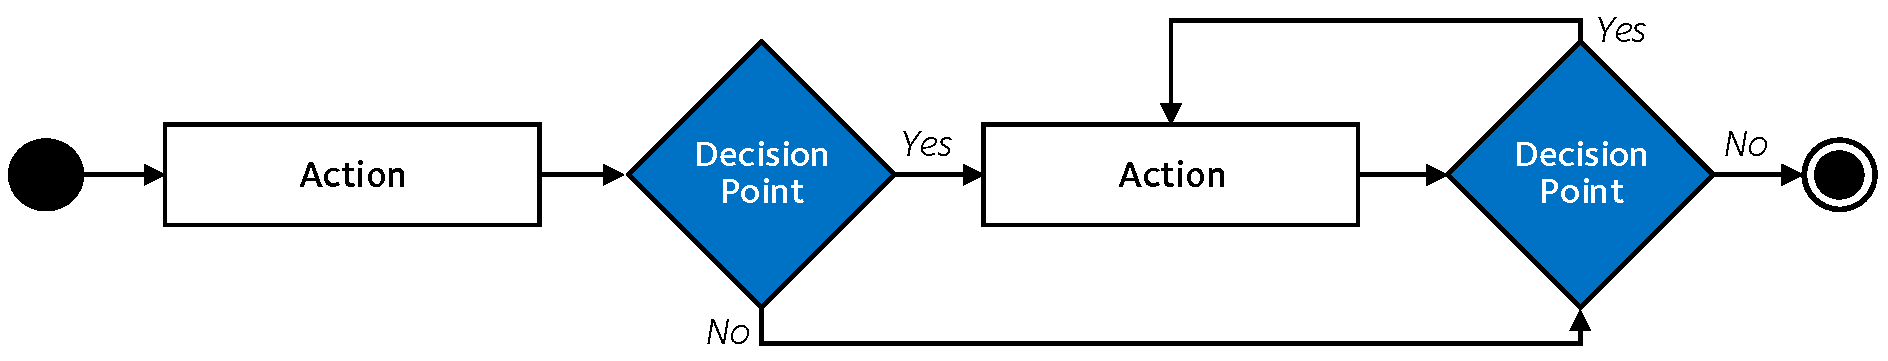
\includegraphics{figures/ch0-example.pdf}}
\end{figure*}

Note that the sequence of events begins with a~
\includegraphics[height=\fontcharht\font`\d]{figures/ch0-example-start.pdf}, and ends at a~
\includegraphics[height=\fontcharht\font`\d]{figures/ch0-example-end.pdf}.\footnote{Note that these symbols are not part of the \href{https://www.iso.org/standard/11955.html}{\texttt{ISO 5807:1985}} standard; they are part of the \emph{Unified Modelling Language (UML)} specification, and have been included to ensure diagrams are simple to understand.} Diagram flow can be deduced by examining the direction of arrows. Actions (or events) are denoted by the text contained within unfilled rectangles~
\includegraphics[height=\fontcharht\font`\d]{figures/ch0-example-action.pdf}, and decision points are represented as~
\includegraphics[height=\fontcharht\font`\d]{figures/ch0-example-decision.pdf}. Outcomes of decisions are denoted by the \emph{italicised} text at each output point of a~
\includegraphics[height=\fontcharht\font`\d]{figures/ch0-example-decision.pdf}.

\end{preamble}